\documentclass[UTF8, zihao=-4]{ctexart} % 字号

\usepackage[colorlinks=false, backref=true]{hyperref} % PDF 目录
\usepackage{graphicx} % 包含图形文件
\usepackage{xcolor} % 颜色
\usepackage{geometry} % 版面边距
\usepackage{fancyhdr} % 定制页眉页脚

% 数学符号
\usepackage{amssymb}
\usepackage{amsmath}
\usepackage{mathrsfs}

\usepackage{multirow} % 多行表格
\usepackage{multicol} % 多列表格
\usepackage{animate} % PDF 动画
\usepackage{tabu} % 高级表格
\usepackage{listings} % 插入代码

\usepackage{extarrows} % 高级箭头
\usepackage[all]{xy} % 交换图表

\usepackage[backend=biber, style = caspervector, utf8]{biblatex}

\geometry{%
  a4paper,%
  top=2.5cm,%
  bottom=2.5cm,%
  left=3.2cm,%
  right=3.2cm%
}

\ctexset {
      section = {
            format = {\large\rm\color{blue}}
      }
}

% 预定义常用数学符号
\newcommand{\real}{\mathbb{R}} % 实数
\newcommand{\realpart}{\text{Re}} % 实部
\newcommand{\comp}{\mathbb{C}} % 复数
\newcommand{\inte}{\mathbb{Z}} % 整数
\newcommand{\nat}{\mathbb{N}} % 自然数
\newcommand{\prob}{\mathbb{P}} % 概率
\newcommand{\expe}{\mathbb{E}} % 期望
\newcommand{\eps}{\varepsilon} % 任意小数
\newcommand{\four}{\mathscr{F}} %Fourier 变换
\newcommand{\co}{\mathcal{O}}
\newcommand{\id}{\text{Id}}
\newcommand{\im}{\text{Im}}
\newcommand{\End}{\text{End}}
\newcommand{\rank}{\text{rank}} % 秩
\newcommand{\proof}{{\itshape 证明.}}
\newcommand{\lcode}{\lstinline} % 段内插入代码

% 小写罗马数字
\newcommand{\rmnum}[1]{\romannumeral #1}

% 定义新函数符号
\DeclareMathOperator*{\argmax}{\arg\,\max}

%mathbb 双透明体 (用于固定空间)
%mathbf 粗体
%mathcal 圆体 (用于算子)
%mathfrak 正体 (用于范畴)
%mathscr 花体 (用于集合系)

%\newtheorem{label}[共享编号来源(环境, 不是计数器)]{标题文本}[父计数器]
\newtheorem{defi}{定义}
\newtheorem{theo}{定理}
\newtheorem{prop}{命题}
\newtheorem{problem}{算例}
\newtheorem{corollary}{推论}
\newtheorem{algorithm}{算法}

\fancypagestyle{plain}{
      \renewcommand{\headrulewidth}{0pt} % width of head line
      \renewcommand{\footrulewidth}{0pt} % clear foot line
      \fancyhf[H]{}
      \fancyhf[FC]{\thepage}
}

\pagestyle{plain}

% 配置代码插入的风格
\lstset {
    language            =   go,                  % 代码语言
    basicstyle          =   \ttfamily,          % 基本代码风格
    keywordstyle        =   \color{blue}, % 关键字风格
    commentstyle        =   \ttfamily,  % 注释的风格,斜体
    stringstyle         =   \bfseries\ttfamily,  % 字符串风格
    flexiblecolumns,                % 别问为什么,加上这个
    %numbers             =   left,   % 行号的位置在左边
    %showspaces          =   false,  % 是否显示空格,显示了有点乱,所以不现实了
    %numberstyle         =   \zihao{-5}\ttfamily,    % 行号的样式,小五号,tt等宽字体
    showstringspaces    =   false,  % 是否显示 string 内部的空格
    captionpos          =   t,      % 这段代码的名字所呈现的位置,t指的是top上面
    frame               =   lrtb,   % 显示边框, none: 不显示.
    breaklines          =   true,   % 自动换行
    columns             =   fixed,   
    basewidth           =   0.5em   % 字宽
}

\title{mbg 游戏引擎说明}
\date{最后更新日期: \today}
\author{滕飞 \\ tfcolin@88.com}

\begin{document}

\maketitle

\section{简介}
\subsection{游戏模式}
mbg 是一款采用 go 语言开发的攻城模式的回合制桌面游戏, 类似 DOS 时代的一款老游戏``富甲天下'', 
实质上是结合了经典的桌面游戏``monopoly''与回合制策略攻城元素. 
游戏主体为一个单路径循环的棋盘. 玩家通过轮流掷骰子获得要行走的
步数, 玩家在不同的棋盘格子可以执行不同的操作, 同时改变玩家的
状态. 在游戏过程中, 玩家可以招募人员, 占领城池. 每占领一个城池
都会为玩家提供每回合的收益. 当玩家 $A$ 移动到玩家 $B$ 所占领的城池时, 
需要向玩家 $B$ 支付过路费. 付费后, 玩家 $A$ 可以选择是否攻城. 
如果攻城成功, 则 $A$ 会从 $B$ 手中抢占该城市. 如果两个玩家
在移动过程中相遇, 还可以发动遭遇战.

游戏的战斗系统为回合制. 双方均需指定一名主将, 并且可选择指定一名副将.
战斗结果由双方将领的属性以及角色所掌握的战斗技能所决定.
每位招募的人员都包含 HP 属性. 
战斗的过程和结果主要体现为更改主将的 HP. 
每回合由双方将领属性随机性的决定一个获胜方, 然后由
获胜方向失败方发动攻击, 正常情况下会对失败方的 HP 造成伤害.
双方还会根据将领属性随机性的发动战斗技能, 不同的战斗技能
会对本回合的战斗结果造成影响. 个别战斗技能还会直接影响角色的属性.
如果防守方主将的 HP 减为零, 则攻方获胜, 否则守方获胜. 如果防守方
驻扎在城市内, 则防守方会在主将 HP 的基础上增加城防. 攻击方优先
对城防造成伤害, 城防减为零后再对守方主将的 HP 造成伤害.

\subsection{系统组成}
本游戏采用规则引擎与用户界面(UI)分离的设计模式. 软件包内包含一个游戏引擎和一个基于 gtk3 的用户界面. 
整个游戏引擎规则包括如下几个系统组成.

\begin{itemize}
    \item 角色系统: 用于描述每位玩家的状态, 包括每位玩家所处的地图位置, 所雇佣的人员和所掌握的战斗技能列表等信息.
    \item 地图系统: 用于描述路径中每个格子的功能和状态. 其中包括如下几种功能的格子.
        \begin{itemize}
            \item 城市: 玩家获得收益的基本功能格子. 只有占领城市才能获得收益.
            \item 会馆: 招募人员的场所.
            \item 谋略研究所: 为玩家研究各种战斗技能的场所.
            \item 修炼所: 为人员进行修炼以提高能力的场所.
            \item 机会: 玩家获得一张卡牌.
        \end{itemize}
    \item 人员系统: 用于描述可供玩家招募的人员的能力和状态. 其中每个人员由如下 $5$ 种基本能力所描述.
        \begin{itemize}
            \item 政治: 当人员作为城市的市长时, 每回合会恢复城市所有驻扎人员的 HP 属性. 市长的政治属性决定恢复的力度.
            \item 经济: 当人员作为城市的财务官时, 每回合会为占领方提供收益. 财务官的经济属性决定获得多少收益.
            \item 武术: 用于决定战斗时每回合的伤害.
            \item 战术: 用于决定战斗时每回合的胜率.
            \item 谋略: 用于决定战斗时特殊技术的发动概率和效果.
        \end{itemize}
    \item 战斗系统: 用于控制战斗过程和战斗结果. 其中包括描述每一种战斗技能的技能系统.
    \item 卡牌系统: 玩家可利用卡牌执行特殊操作.
\end{itemize}

\subsection{游戏流程}
\label{s_process}
每个回合, 所有玩家角色依次行动一次. 每次行动可包含如下动作.
\begin{itemize}
    \item 查看角色状态, 包括所属人员, 占领城市, 在谋略研究所所从事的研究项目, 和在修炼所所从事的修炼项目.
    \item 角色选择卡牌使用, 每回合使用卡牌的数量不限. 
    \item 通过掷骰子以及角色的移动相关属性 (参见第 \ref{s_role} 节) 决定移动步数. 
    \item 如果移动过程中遇到强盗或障碍 (由卡牌设定, 参见第 \ref{s_card} 节), 则终止本轮移动. 对于强盗情形, 进入战斗模式.
    \item 根据目的地类型决定不同效果.
        \begin{itemize}
            \item 城市:
                \begin{itemize}
                    \item 空城市: 决定是否占领城市, 若占领需至少派驻一名人员. 可选择设置市长和/或财务官.
                    \item 己方占领城市: 获得额外收益, 同时可选择调换身边的人员和城市驻扎的人员, 可选择变更市长和/或财务官.
                    \item 敌方占领城市: 支付税金. 同时可选择是否发动攻城战斗, 以及战斗的规模, 详见 \ref{s_battle} 节的描述.
                        \begin{itemize}
                            \item 如果攻城成功, 则该城市的所有敌方进驻人员撤回到敌方角色身边. 
                                然后按照空城市的处理方法由胜利玩家选择是否占领城市及占领人员和职务.
                        \end{itemize}
                \end{itemize}
            \item 会馆: 随机从三个档次的闲置人员中产生一名人员, 由玩家选择最多一名人员招募至玩家阵营, 并支付招募费.
                新招募的人员会立刻跟随在玩家身边.
            \item 谋略研究所:
                \begin{itemize}
                    \item 已有己方人员进驻该研究所: 无操作.
                    \item 无己方人员进驻该研究所: 可选择人员进驻并研究一项未掌握的战斗技能.
                \end{itemize}
            \item 修炼所:
                \begin{itemize}
                    \item 已有己方人员进驻该修炼所: 无操作.
                    \item 无己方人员进驻该修炼所: 可选择人员进驻并修炼一项该人员的基本能力.
                \end{itemize}
            \item 机会: 玩家随机获得一张卡牌, 详见第 \ref{s_card} 节的描述.
        \end{itemize}
\end{itemize}

当一个完整回合结束时, 会进行回合结算, 结算的内容包括:
\begin{itemize}
    \item 对各研究所的战斗技能研究状态进行更新.
    \item 对各修炼所的人员能力修炼状态进行更新.
    \item 恢复各城市的防御和驻扎人员的 HP.
    \item 各角色从所有占领城市获得固定收入.
    \item 更新所有人员的特殊状态, 包括流言状态, 中毒状态, 是否离职. 详见第 \ref{s_people} 节的描述.
\end{itemize}

每当回合数被常数 \lcode{ALLOCATE_TURN} 整除, 会进入调度流程. 在调度流程中, 按角色顺序, 每位角色可选择执行如下操作.
\begin{itemize}
    \item 变更所占领城市的市长和财务官
    \item 让某所属人员从驻扎的城市离开回到角色身边. 
        \begin{itemize}
            \item 注意如果某占领城市的所有驻扎人员全部撤离该城市, 则自动视为放弃对该城市的占领.
        \end{itemize}
    \item 让某角色身边人员驻扎到某已占领城市.
    \item 取消某谋略研究所的研究. 让研究人员返回角色身边.
    \item 让驻扎在某修炼所的修炼人员终止修炼并返回角色身边.
\end{itemize}

当回合结束时, 会对角色的胜负状态进行判定. 如果一个角色的资产为负, 则判定角色失败出局. 
此时, 该角色所有的所属人员均变更为未被招募状态, 所有占领城市均变为未占领状态,
所有的谋略研究和修炼均撤销. 如果除了一名游戏角色外, 其他角色均已经失败出局, 
则该剩余角色获胜, 游戏结束. 如果某位角色的资产达到事先设定的胜利资产标准, 则
当前资产最高的角色获胜, 游戏结束. 
%如果此时有不至一名角色拥有最高资产, 则游戏以平局结束.
如果不止一个角色在同一个回合全部失败出局, 而导致局面上已经没有任何生存角色, 则游戏以平局结束.
用户在建立游戏时, 还需指定最大回合数. 当回合数达到最大时, 游戏结束, 此时拥有最高资产量的角色获胜.

\subsection{编译运行}
\label{s_compile}
用户可通过如下 git 指令下载游戏的源代码.
\begin{lstlisting}[language=bash]
git clone https://gitee.com/tfcolin/mbg.git
\end{lstlisting}

用户首先需要编译程序(假设代码路径为 mbg/)
\begin{lstlisting}[language=bash]
cd mbg/
go build .
cd gtk3ui
go build .
cd ../mbg_gtk
go build .
cd ..
\end{lstlisting}

完成编译后, 用户可进入到 mbg\_gtk 目录.
有两种方式可启动游戏. 一是重头开始游戏, 此时可执行 
\begin{lstlisting}[language=bash]
mbg_gtk xxx.map
\end{lstlisting}
其中, xxx.map 为事先定义好的游戏规则文件, 目前的软件包内包含 ``sanguo.map'' 作为示例.
关于 .map 文件内容的详细说明可参考第 \ref{s_mfile} 节.

另一种启动游戏的方式是载入之前存储的进度文件, 启动方式为
\begin{lstlisting}[language=bash]
mbg_gtk yyy.sav
\end{lstlisting}
其中, yyy.sav 为之前保存的进度文件.
程序会根据所提供文件名的后缀 (.map 还是 .sav) 来判定以哪种情形启动引擎.

\section{图形用户界面}
\label{s_gui}
本节简要介绍一下游戏中包含的基于 gtk3 的图形用户界面.
游戏的主界面如图 \ref{f_main} 所示. 左上部分最大的区域为主区域, 为供玩家角色行进的场所.
其中每个位置绘制了四个按钮, 最内侧的按钮表示该位置的建筑名称, 
上面的按钮则分别表示每个角色的行进路线, 每个角色只能在其中一排
内移动, 从而多个角色可以位于同一位置. 中间部分的右侧和下侧包含滚动条.
\begin{figure}
    \centering
    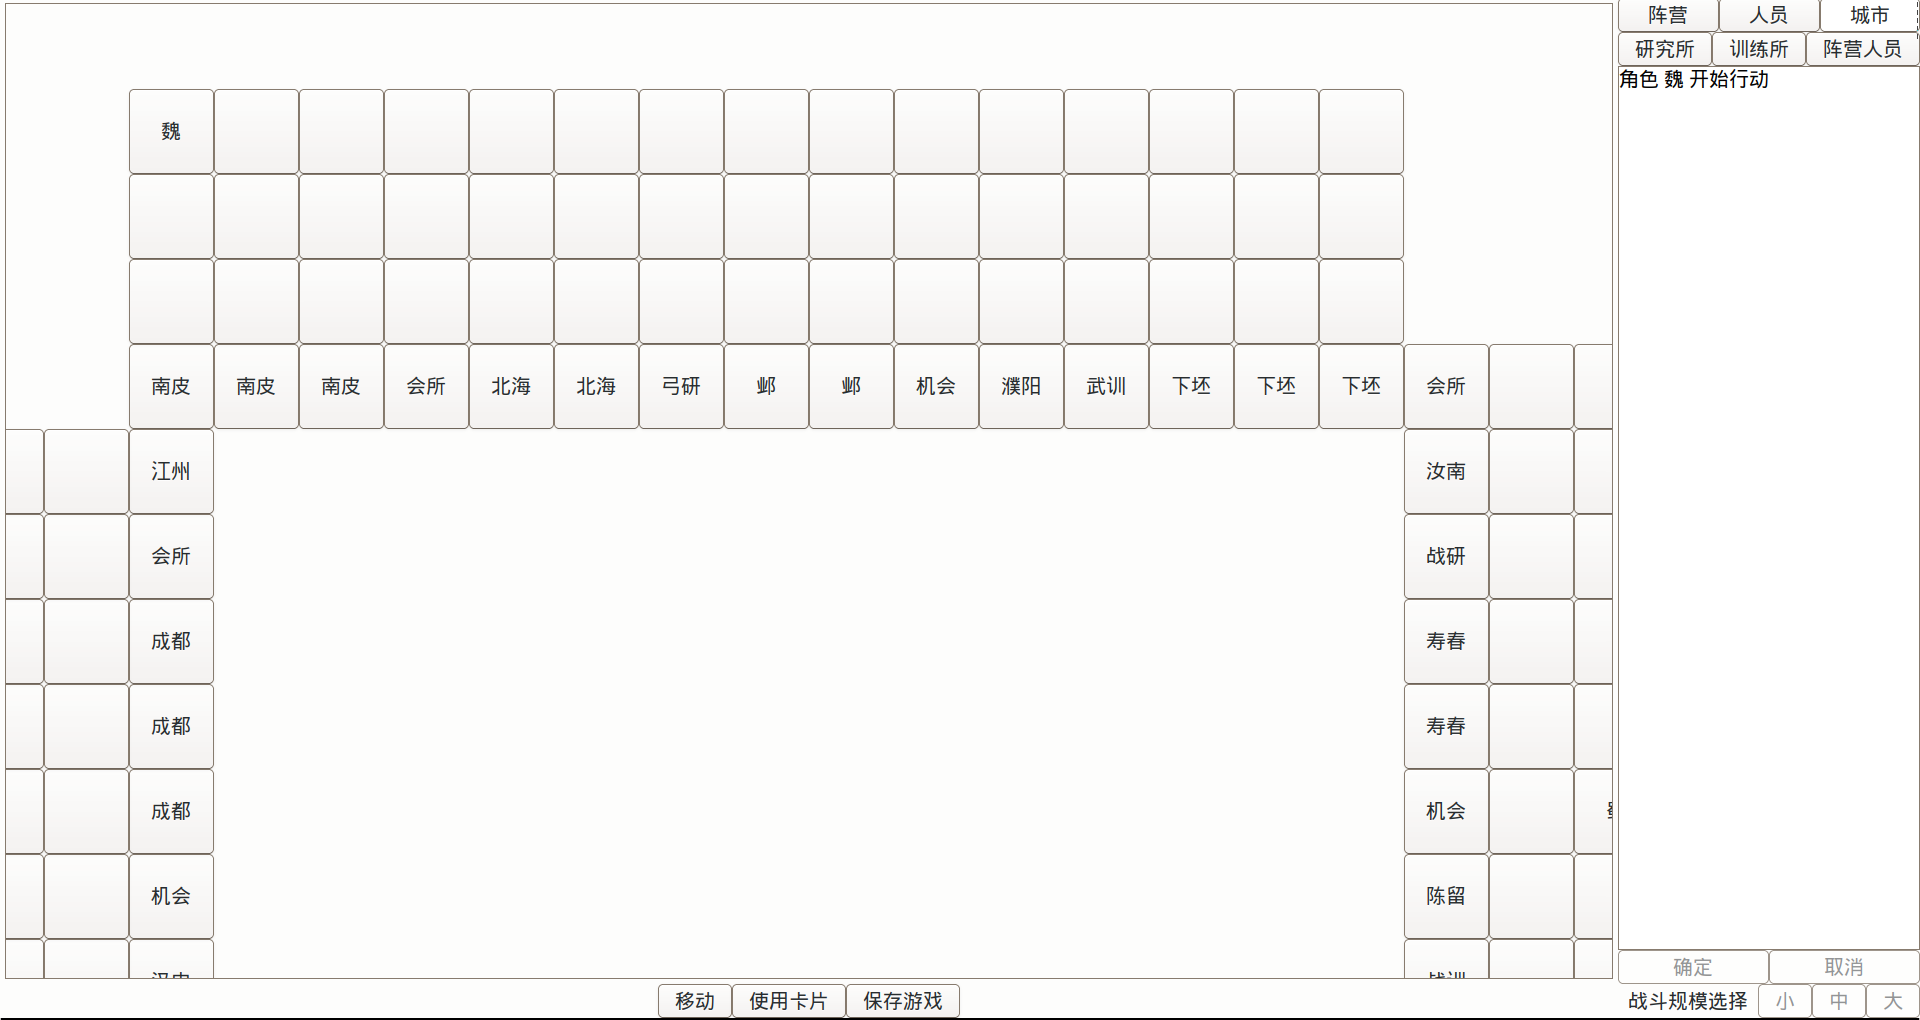
\includegraphics[width=\textwidth]{f_main.png}
    \caption{\label{f_main}游戏主界面}
\end{figure}
界面的右上角为信息查询区, 用于用户查询信息. 
右侧为信息提示区, 用于展示游戏进程的说明和引擎发送给用户的信息. 其中包括确定和取消按钮用于当
引擎询问用户时, 用户给出反馈. 最右下角为战斗规模选择区, 用于用户在准备发动战斗时选择战斗规模.
下部为用户指令区, 用户可向角色下达移动或使用卡片的指令, 也可中途保存游戏进度. 
当选择移动指令时, 角色的位置会在主区域发生改变. 当选择使用卡片指令时, 系统会
打开如图 \ref{f_cards} 所示的卡片界面以供角色选择要使用的卡片.
\begin{figure}
    \centering
    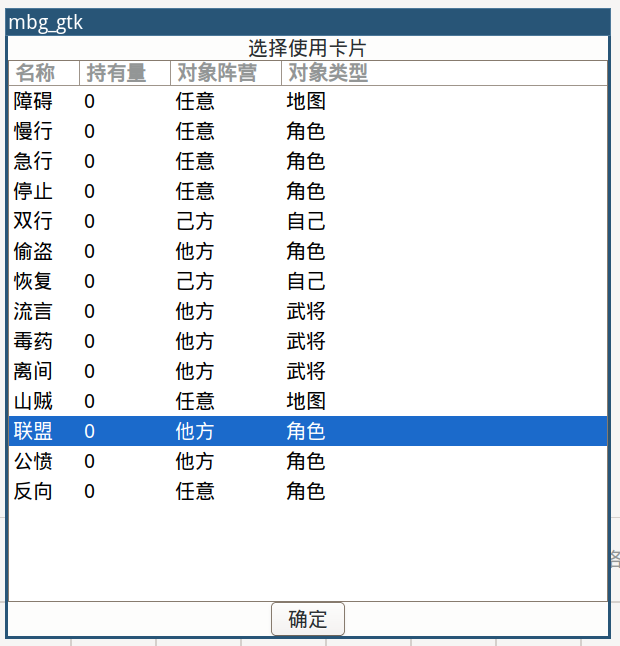
\includegraphics[width=\textwidth]{f_cards.png}
    \caption{\label{f_cards}游戏主界面}
\end{figure}

用户可通过点击右上角的按钮查询信息. 
阵营按钮用于查询角色信息, 如图 \ref{f_role} 所示. 
在最上部选择一个角色阵营, 然后点击查看阵营细节, 可在下部各列表框中显示
阵营所占领的城市和各类所属人员, 玩家可继续在城市列表中选择一个城市,
然后点击查看城市人员, 则可显示该城市的所有占领人员的列表.
\begin{figure}
    \centering
    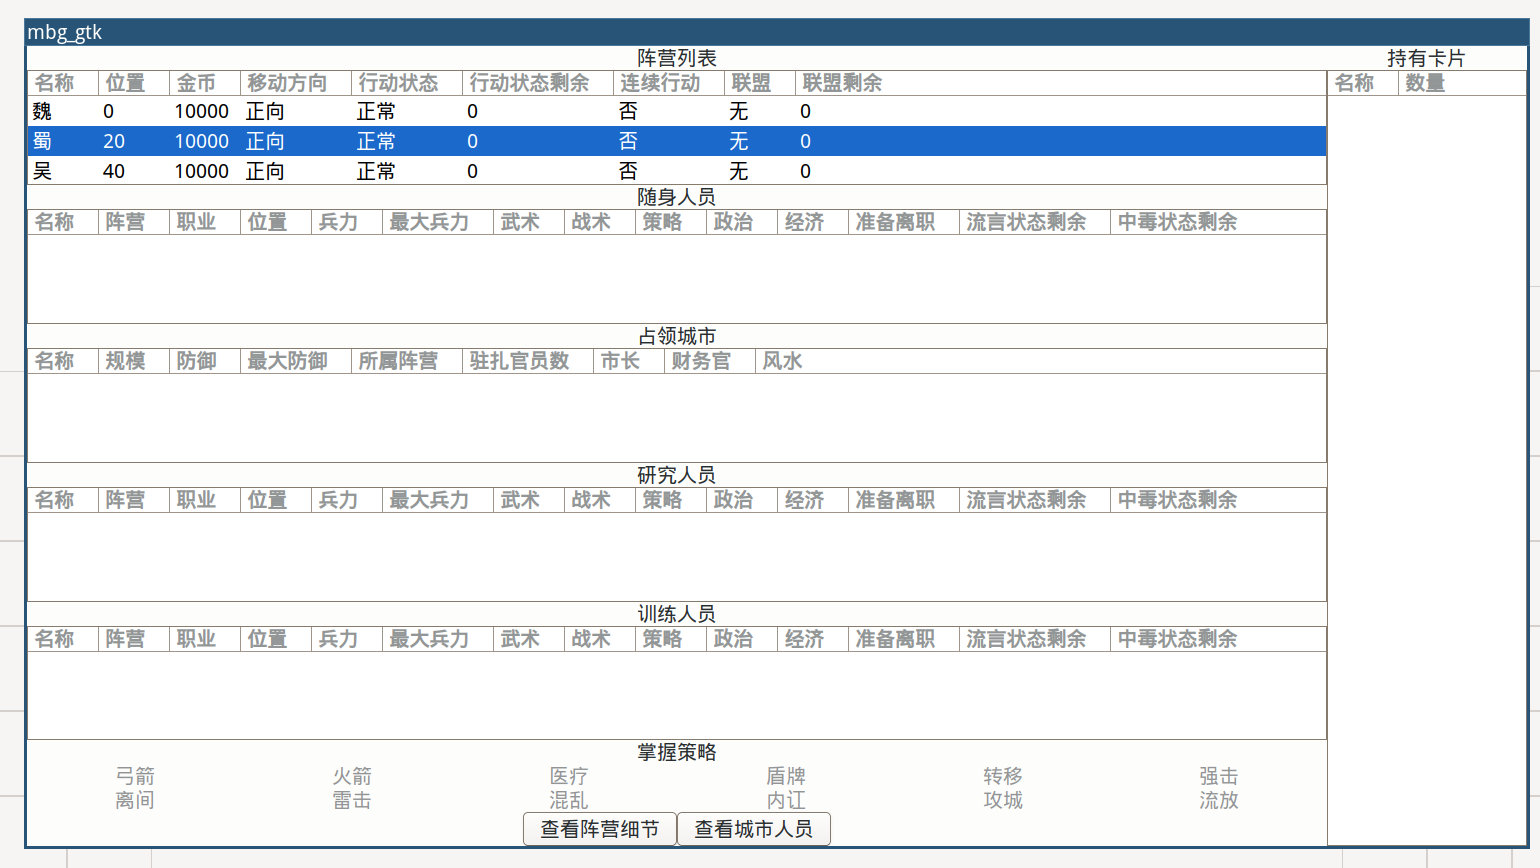
\includegraphics[width=\textwidth]{f_role.png}
    \caption{\label{f_role}查看角色阵营的信息}
\end{figure}

类似的, 点击人员可以查看游戏中的所有人员的信息. 点击城市可查看所有城市的信息.
点击研究所和训练所则分别可查看游戏中的所有谋略研究所和修炼所. 
点击阵营人员可查看当前行动中的角色阵营的所有人员列表. 分别如图 \ref{f_people}, \ref{f_city},
\ref{f_inst}, \ref{f_train} 所示.
\begin{figure}
    \centering
    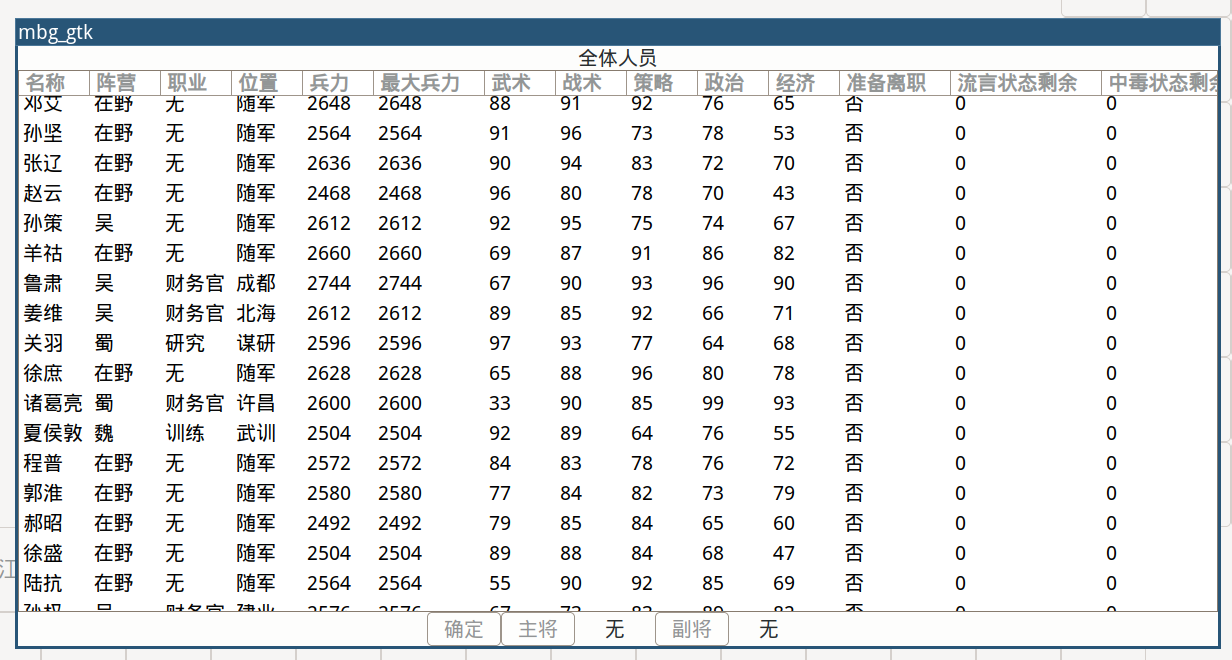
\includegraphics[width=\textwidth]{f_people.png}
    \caption{\label{f_people}查看所有人员信息}
\end{figure}
\begin{figure}
    \centering
    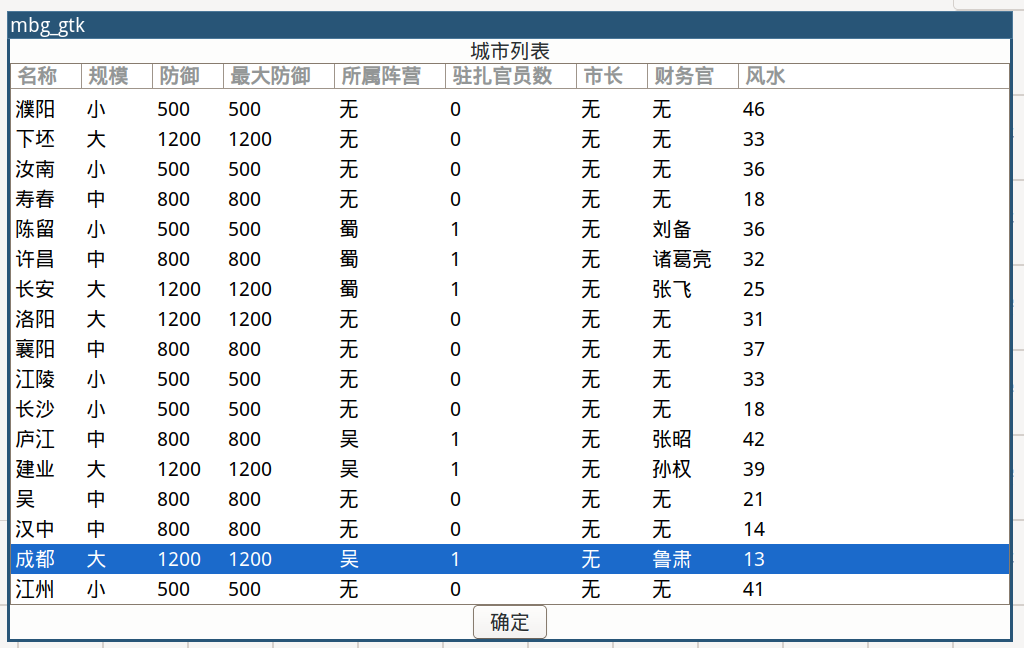
\includegraphics[width=\textwidth]{f_city.png}
    \caption{\label{f_city}查看城市信息}
\end{figure}
\begin{figure}
    \centering
    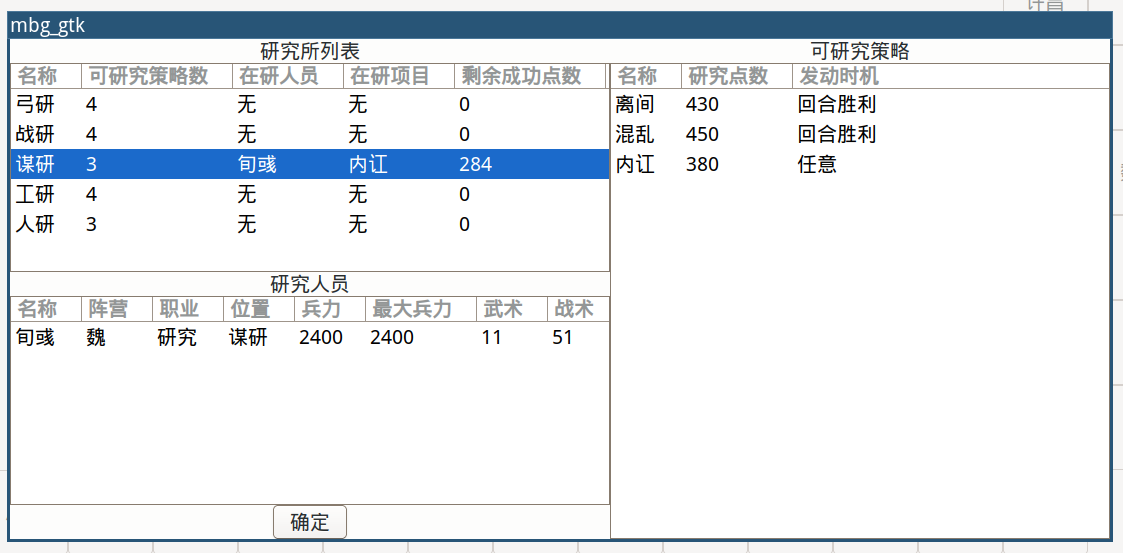
\includegraphics[width=\textwidth]{f_inst.png}
    \caption{\label{f_inst}查看所有谋略研究所}
\end{figure}
\begin{figure}
    \centering
    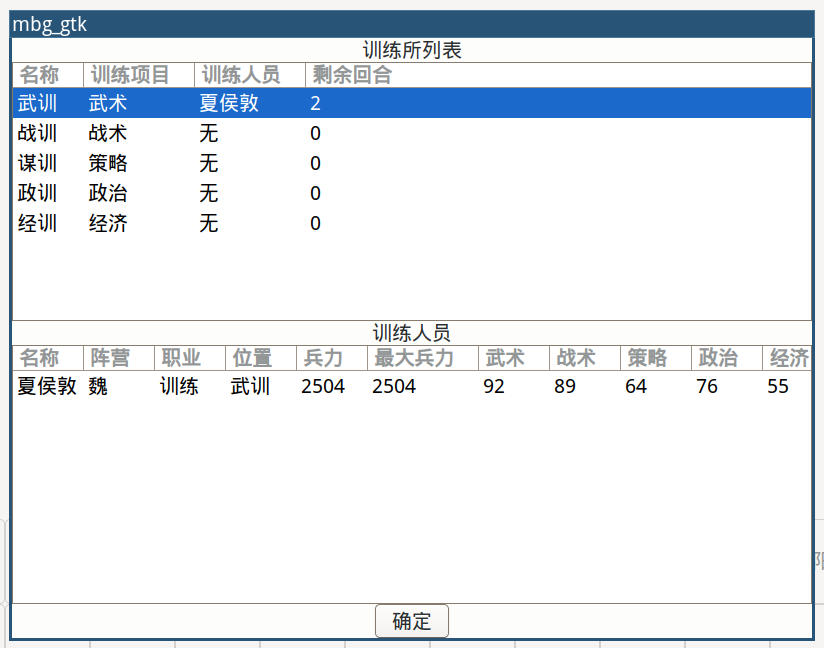
\includegraphics[width=\textwidth]{f_train.png}
    \caption{\label{f_train}查看所有修炼所}
\end{figure}

如图 \ref{f_cross_city} 所示, 当角色经过对手所占领的城市时, 需支付税金,
然后选择是否发动战斗. 
\begin{figure}
    \centering
    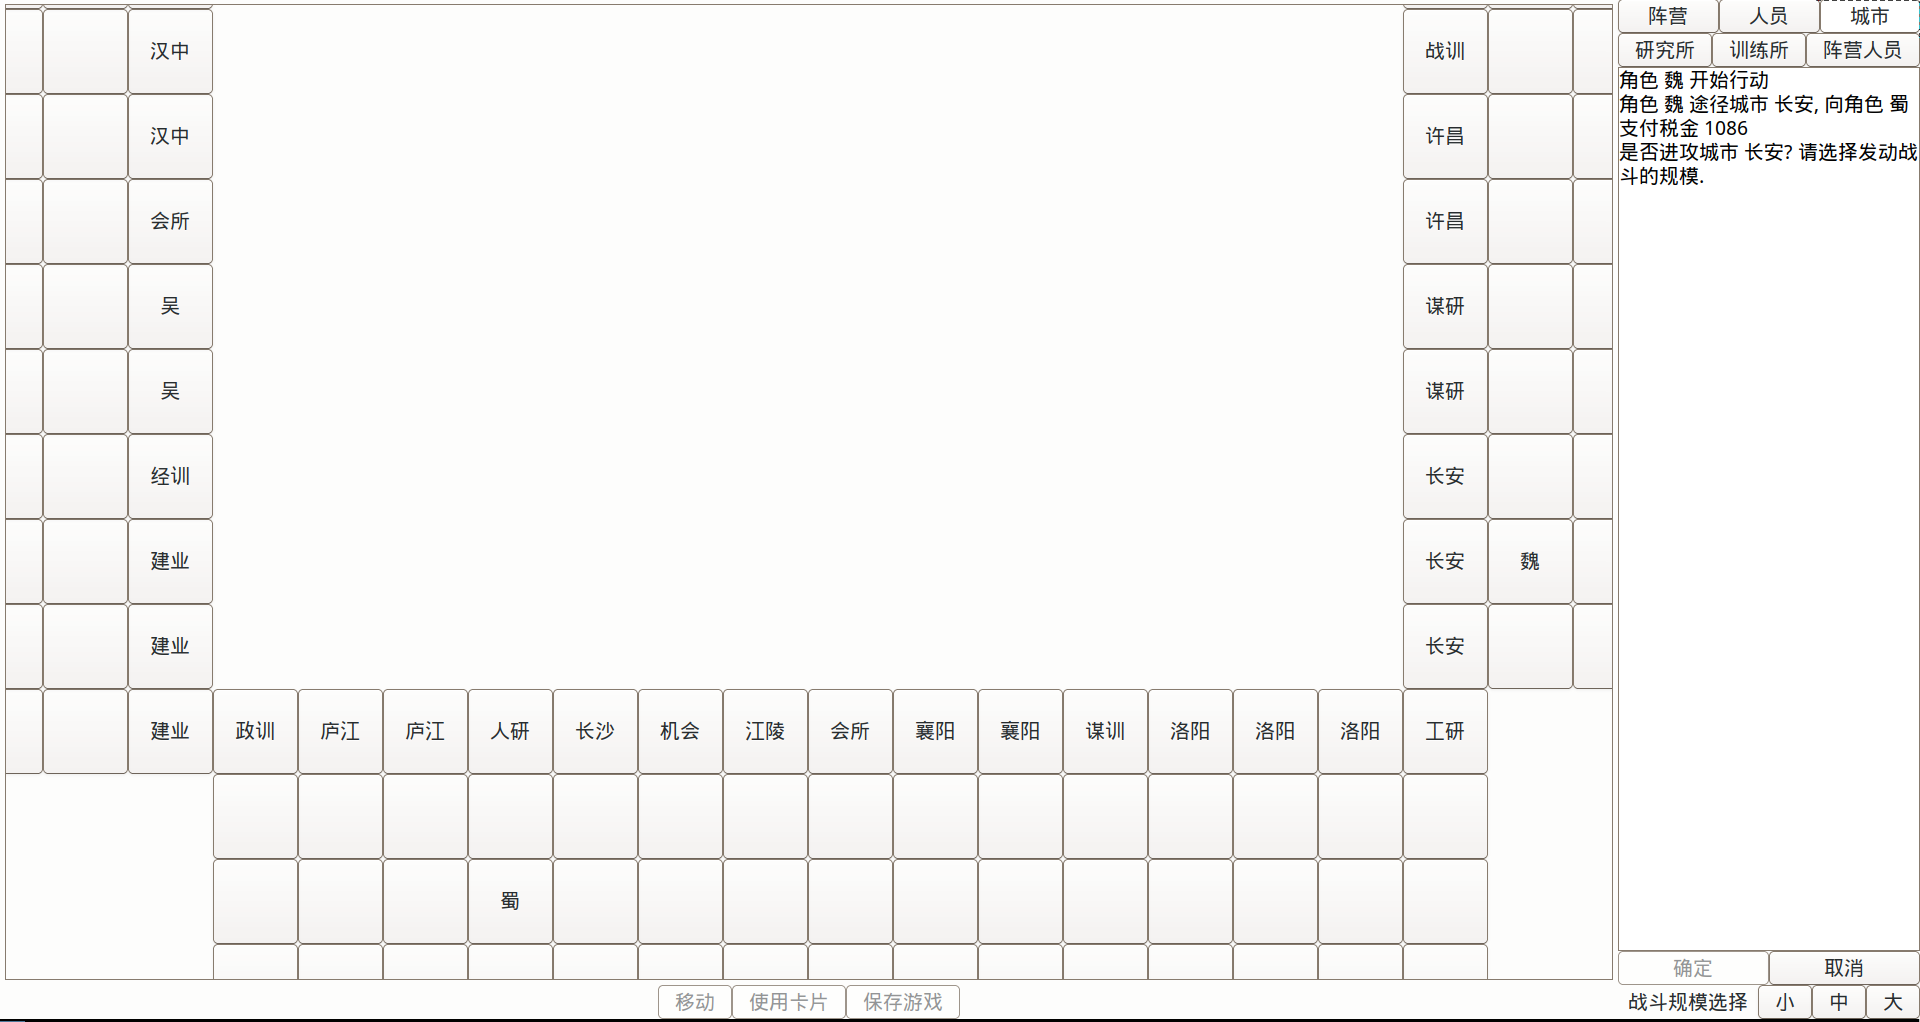
\includegraphics[width=\textwidth]{f_cross_city.png}
    \caption{\label{f_cross_city}查看所有修炼所}
\end{figure}
当发动战斗时, 首先需要发动方选择一个战斗规模 (右下角), 然后双方分别选择
将领, 进而进入战斗对话框, 如图 \ref{f_battle} 所示.
最上部为战斗双方的能力属性, 下面为双方可发动的战斗技能, 显示为灰色为不可用.
再下面为战斗双方在当前回合的状态, 再下面为消息框, 用于提示战斗进程.
最下面有两个按钮, 左边的按钮可让战斗进行一回合. 而右边的按钮为一个单选钮, 
如果被按下, 则战斗会持续进行, 直到取消该按钮或战斗结束. 图 \ref{f_battle_res}
展示了战斗结束时的画面.
\begin{figure}
    \centering
    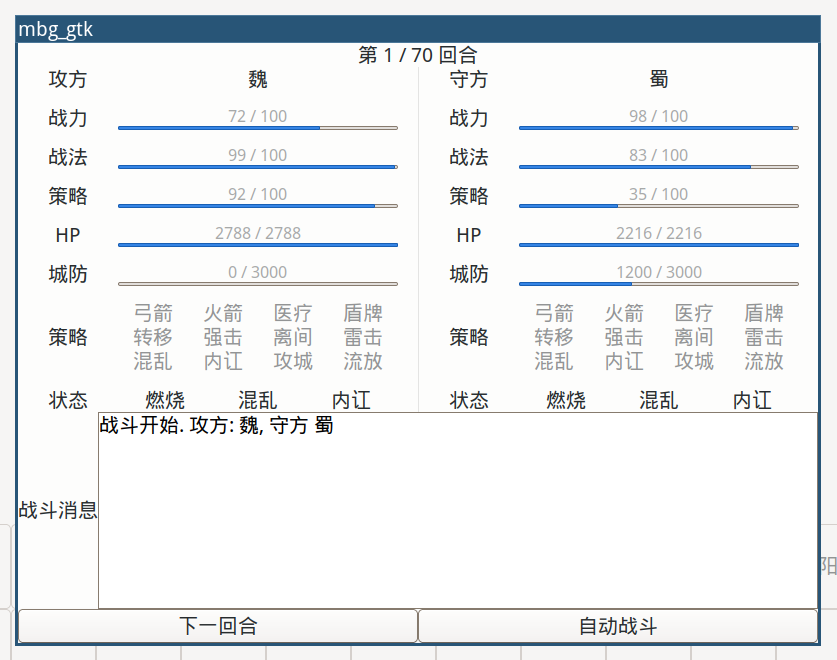
\includegraphics[scale=0.4]{f_battle.png}
    \caption{\label{f_battle}游戏主界面}
\end{figure}
\begin{figure}
    \centering
    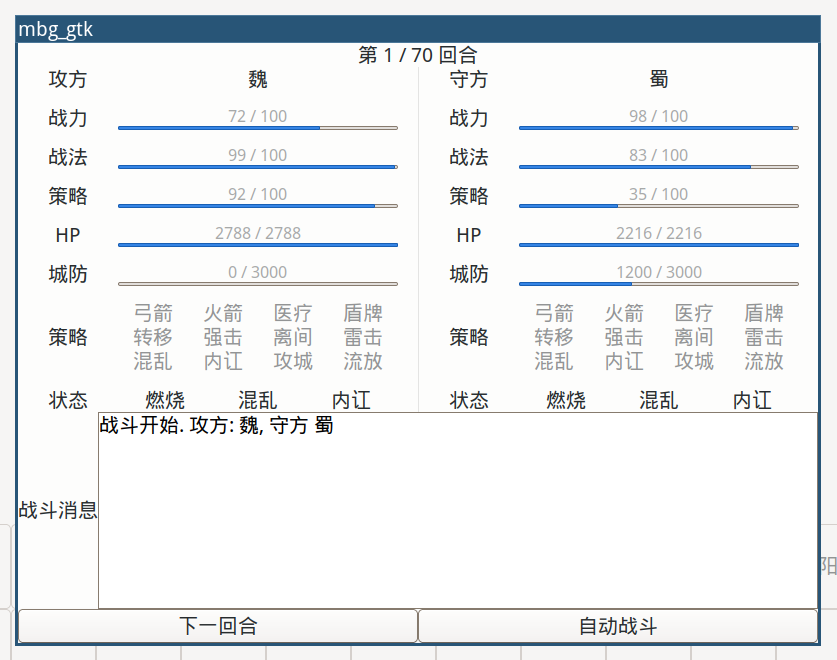
\includegraphics[scale=0.4]{f_battle.png}
    \caption{\label{f_battle_res}游戏主界面}
\end{figure}

\section{各系统的规则}
\label{s_driver}
本节主要阐述游戏各子系统的详细规则. 在代码中, 我们使用大写标识符表示对整个引擎不变的常量.
所有常数的取值列于第 \ref{s_const} 节中.
首先, 整个游戏的运行状态由一个 Driver 结构类型的变量所描述. 具体定义为:
\begin{lstlisting}
type Driver struct {
	cities []City
	insts  []Institute
	trains []TrainingRoom
	board  []BoardPoint
	people []Officer
	roles  []Role

	lpset [3](*dsg.Set) // people level set 0:2 低中高

	ngrid   int
	nrole   int
	npeople int
	ncity   int
	ninst   int
	ntrain  int

	uv UserView
	oi []OperationInterface

	turn      int
	win_money float32

	nx, ny int
}
\end{lstlisting}
其中, \lcode{cities, insts, trains, board, people, roles} 为各子系统的数组列表, 用于描述各子系统的对象. 
分别代表所有城市, 所有谋略研究所, 所有修炼所, 所有地图格子, 所有人员以及所有角色.
\lcode{ngrid, nrole, npeople, ncity, ninst, ntrain} 则分别为地图中格子, 角色, 人员, 城市, 谋略研究所和修炼所的总个数.
基于上述数组, 当引擎中有变量需要引用到上述各类对象时, 该变量均取值为上述数组的下标索引整数. 因为可方便地通过上述数组找到该对象.
\lcode{lp_set} 由 $3$ 个集合组成, 用于对所有人员进行分类. 人员按能力的高低将被分为低, 中, 高三类.
具体分类规则见第 \lcode{s_people} 节的描述.

\lcode{uv} 和 \lcode{oi} 为与用户界面的接口, 其中 \lcode{uv} 表示唯一的通知接口, 用于
让游戏引擎通知 UI 显示一些输出信息. \lcode{oi} 数组则是对每一位角色定义一个接口, 
用于从 UI 接收每个角色的操作指令. \lcode{turn} 为当前回合数.
\lcode{win_money} 为游戏的胜利判定资产, 详见第 \ref{s_process} 节的描述.
\lcode{nx, ny} 与游戏引擎无关, 仅用于 UI 在绘制地图时平面的两个维度以格子数所衡量的大小.

以下函数用于获取游戏引擎相关的信息.
\begin{lstlisting}
func (d *Driver) GetInfo() (ngrid, nrole, npeople, ncity, ninst, ntrain, turn, nx, ny int)
func (d *Driver) GetPeople(i int) *Officer 
func (d *Driver) GetBoard(i int) *BoardPoint 
func (d *Driver) GetRole(i int) *Role 
func (d *Driver) GetCity(i int) *City 
func (d *Driver) GetInst(i int) *Institute 
func (d *Driver) GetTrain(i int) *TrainingRoom 
func (d *Driver) GetFreePeopleList(level int) []int 
\end{lstlisting}
各函数的含义如函数名称所示, 用于获取引擎包含的对应类型的对象, 其中的参数 \lcode{i} 为对应对象数组中的下标顺序编号. 
\lcode{GetInfo} 用于获取引擎包含各类对象的个数, 回合数等信息. \lcode{GetFreePeopleList} 用于获取处于当前级别的所有
未被雇佣人员的编号列表. \lcode{level} 代表级别, 取值 $0, 1, 2$, 分别代表低, 中, 高三个级别.
以下, 我们假设以定义好如下变量 \lcode{d} 来表示整个游戏引擎.
\begin{lstlisting}
var d Driver
\end{lstlisting}

\begin{lstlisting}
func LoadMap(mfile io.Reader) (d *Driver)
\end{lstlisting}
用于从一个关卡描述文件中建立并初始化整个引擎, \lcode{mfile} 表示打开的关卡描述文件, 其详细含义参见第 \ref{s_mfile} 节的描述.
\begin{lstlisting}
func (d *Driver) Save (fout io.Writer, crole int) 
\end{lstlisting}
用于保存整个游戏进程, 其中 \lcode{crole} 为当前正在操作的角色编号, \lcode{fout} 指明保存的文件.
\begin{lstlisting}
func (d *Driver) Load(fin io.Reader) (crole int)
\end{lstlisting}
用于读取整个游戏进程, 其中 \lcode{crole} 为当前正在操作的角色编号, \lcode{fin} 指明从哪个文件中读取. 该文件必须为之前通过调用 \lcode{Save} 保存的文件.
\begin{lstlisting}
func (d *Driver) ConnectUI(uv UserView, oi []OperationInterface)
\end{lstlisting}
用于将引擎与用户界面相关联, 用户界面接口的详细定义可参见第 \ref{s_ui} 节.
\begin{lstlisting}
func (d *Driver) Run (max_turn int, crole int) int
\end{lstlisting}
用于启动游戏引擎, 其中 \lcode{max_ture} 用于指明游戏的最大回合数, \lcode{crole} 用于指明当前的操作角色.

mbg\_test.go 为测试游戏引擎的使用范例, 如以下代码所示.
\begin{lstlisting}
import (
	"os"
      "mbg"
)

func main() {

	mbg.Init()
	fin, _ := os.Open("test_game.map")
	d := mbg.LoadMap(fin)
	fin.Close()

      _, nrole, _, _, _, _, _, _, _ := d.GetInfo()

	var uv mbg.TestUserView
	var oi_ []mbg.TestOperationInterface
	var oi []mbg.OperationInterface
	oi_ = make([]mbg.TestOperationInterface, nrole)
	oi = make([]mbg.OperationInterface, nrole)

	for i := 0; i < nrole; i++ {
		oi[i] = &(oi_[i])
	}

	d.ConnectUI(&uv, oi)

	d.Run(10, 0)

}
\end{lstlisting}
其中 \lcode{Init} 用于初始化一些引擎常数. \lcode{LoadMap} 用于通过关卡文件建立引擎. 
\lcode{uv} 和 \lcode{oi} 分别为由 UI 设计者所定义的用户通知接口和每位玩家的用户操作接口. 通过调用 \lcode{ConnectUI} 函数将其与引擎相连接.
最后调用 \lcode{Run} 函数来启动引擎. 如果玩家之前保存了游戏, 也可用 
\begin{lstlisting}
d := new (mbg.Driver)
crole := d.Load (fin)
\end{lstlisting}
替换掉
\begin{lstlisting}
d := mbg.LoadMap(fin)
\end{lstlisting}
来读取载入用户保存的游戏.

\subsection{角色系统}
\label{s_role}
在本游戏中, 每个角色代表一名玩家, 角色的属性用于描述玩家的所有状态, 角色的所有属性定义如下.
\begin{lstlisting}
type Role struct {
	name  string
	loc   int      // -1: 不出场
	tech  *dsg.Set // 掌握技术
	mos   *dsg.Set // 随身人员
	mcs   *dsg.Set // 占领城市
	sos   *dsg.Set // 研究人员
	tos   *dsg.Set // 训练人员
	money float32  // 财产
	dir   int      // 行动方向: 1: 正向. -1: 反向

	mst   int  // 行动状态: 0: 正常, 1: 慢行. 2: 急行. 3: 禁行.
	mtime int  // 行动状态剩余时间
	cst   bool // 是否连续行动
	ast   int  // 结盟状态: -1: 未结盟. -2: 公愤. 0-? 结盟对象
	atime int  // 结盟剩余时间

	cards [CARD_COUNT]int // 卡片
}
\end{lstlisting}

其中, \lcode{name} 为角色的名称. \lcode{loc} 为角色所在地图中的位置, $-1$ 表示角色已经失败出局.
\lcode{dsg.Set} 为一个整数集合类型. \lcode{tech} 为角色所掌握的所有技术集合.
\lcode{mos} 为角色的所有随身雇佣人员集合. \lcode{mcs} 为角色的所有占领城市的集合.
\lcode{sos} 为角色所有驻扎于谋略研究所从事技术研究的人员集合.
\lcode{tos} 为角色所有驻扎于修炼所从事能力修炼的人员集合.
所有集合都取值为对应类型对象的整数编号. \lcode{money} 表示角色当前的资产数额.

\lcode{dir} 表示角色的移动方向, 只能取 $1$ 或 $-1$ 两个方向 .
\lcode{mst} 表示角色的移动状态, 共有四种. 
\begin{itemize}
    \item $0$ 表示正常移动, 此时的最大移动步数为常数 \lcode{MAX_STEP}.
    \item $1$ 表示慢速移动, 此时的最大移动步数为常数 \lcode{int(MAX_STEP / SLOW_SCALE)}.
    \item $2$ 表示快速移动, 此时的最大移动步数为常数 \lcode{int(MAX_STEP * FAST_SCALE)}.
    \item $3$ 表示禁止移动, 此时角色只能原地停留.
\end{itemize}
\lcode{mtime} 表示上述移动状态的剩余持续时间 (回合数). 
\lcode{cst} 表示角色在本次行动完成后, 可以再连续行动一次. 
\lcode{ast} 表示角色与其他角色的关系. 共可取三种类型的值.
\begin{itemize}
    \item $-1$: 未结盟状态, 即和所有角色保持正常关系.
    \item $\ge 0$: 表示和某位其他角色结盟. 当一名角色移动到与之结盟角色所驻扎的城市时, 无法发生攻城战斗, 
        但仍需支付过路费. 当两名结盟角色相遇时, 无法发动遭遇战. 
        每位角色只能与其他一名角色结盟, 并且结盟关系是对称的, 即 $A$ 与 $B$ 结盟同时代表 $B$ 与 $A$ 结盟.
        在一项盟约终止前, 角色无法再和另外的角色缔结盟约. 处于公愤状态的角色无法缔结盟约.
    \item $-2$: 表示该角色处于公愤状态. 处于该状态的角色只要停留在任何其他角色的城市处, 就必然
        与该城市发生攻城战斗, 无法选择. 任何其他角色只要经过公愤角色所占领的城市, 也必然发动攻城战斗, 无法选择.
        任何角色与公愤角色在路上相遇, 必然发生遭遇战. 在与其他角色的盟约终止前, 角色无法进入公愤状态. 
        但目前此处存在一个规则漏洞, 因为战斗的发动方可以通过不选择出战将领而强制不发动战斗而提前战败.
        而通常这种战败不会造成任何损失.
\end{itemize}
\lcode{atime} 表示角色结盟或公愤状态的剩余持续时间. \lcode{cards} 数组记录了角色所拥有的每一种机会卡片的数量.
共有 \lcode{CARD_COUNT} 种机会卡片. 
角色的 \lcode{dir, mst, mtime, cst, ast, atime} 属性均只能通过使用卡片来改变, 参见第 \ref{s_card} 节的描述. 

函数 
\begin{lstlisting}
func (d *Driver) GetRoleInfo(rind int) (
	name string,
	loc int, // -1: 不出场
	tech []int, // 掌握技术
	mos []int, // 随身人员
	mcs []int, // 占领城市
	sos []int, // 研究人员
	tos []int, // 训练人员
	money float32, // 财产
	dir int, // 行动方向: 1: 正向. -1: 反向

	mst int, // 行动状态: 0: 正常, 1: 慢行. 2: 急行. 3: 禁行.
	mtime int, // 行动状态剩余时间
	cst bool, // 是否连续行动
	ast int, // 结盟状态: -1: 未结盟. -2: 公愤. 0-? 结盟对象
	atime int, // 结盟剩余时间
	cards []int,
) 
\end{lstlisting}
用于获取角色的各项信息.

\subsection{地图系统}
\label{s_board}
地图系统包括几个用于描述特定类型地块的结构, 分别为
\begin{description}
    \item [BoardPoint] 用于描述每个地图位置格子.
    \item [City] 用于描述城市.
    \item [Institute] 用于描述谋略研究所.
    \item [TrainingRoom] 用于描述修炼所.
\end{description}
以下将详述每个结构.

\subsubsection{地图位置}
每个地图位置由如下结构所定义.
\begin{lstlisting}
type BoardPoint struct {
	class   int // 0: 空地 1:城 2:会馆 3:谋略研究所 4:修炼所 5: 机会
	base    int
	roles   []bool
	barrier bool
	robber  bool
	x, y    int
}
\end{lstlisting}
其中, \lcode{class} 为地块的类型, 具体含义如代码注释所述. 
\lcode{base} 表示该地块在所属 \lcode{class} 类型地块中对应引擎数组的顺序编号.
例如, 如果 \lcode{d.board[loc].class} 为 $1$, 则通过 \lcode{d.cities[d.board[loc].base]} 可找到该地块所代表的城市.
其中, \lcode{var d Driver} 表示整个游戏引擎, 参见第 \ref{s_driver} 节的描述.
如果 \lcode{d.board[loc].class} 为 $3$, 则通过 \lcode{d.insts[d.board[loc].base]} 可找到该地块所代表的谋略研究所.
\lcode{roles} 为大小为 \lcode{d.nrole} 的数组, 记录每个角色是否位于该地块. 每个地块可同时容纳多个角色.
\lcode{barrier} 为 \lcode{true} 表示该位置存在一个路障, 当任何角色经过该位置时, 会强制其终止移动, 
同时路障解除. \lcode{robber} 表示该位置存在一个强盗, 当任何角色经过该位置时, 
会强制其终止移动, 同时强制发动对强盗的战斗. 战斗结束后, 强盗自动消失. 
如果角色未能取胜, 则需要向强盗支付 \lcode{ROBBER_STEAL} 的资金.
路障和强盗均由特定卡牌来设定. 
注意游戏中的功能设施包括城市, 谋略研究所和修炼所几种. 每个功能设施的位置可能跨越不止一个地图格子.
即允许多个地图格子的 \lcode{class} 和 \lcode{base} 属性完全相同. 当玩家角色停留在其中任何一个格子中, 
都示为玩家到达了相应设施所在的位置.

\lcode{x, y} 与引擎无关, 仅用于辅助 UI 决定格子在二维界面上的坐标.
函数
\begin{lstlisting}
func (d *Driver) GetBoardInfo(ind int) (class int, base int, roles []bool, barrier bool, robber bool)
\end{lstlisting}
用于获取一个地图位置的信息.

\subsubsection{城市}
如下 \lcode{City} 结构用于描述城市.
\begin{lstlisting}
type City struct {
	name           string
	scope          int // 0:小 1:中 2:大
	hpmax          float32
	hp             float32
	role           int      // -1: 未被占领
	mos            *dsg.Set // 占领人员 (Empty: 未被占领)
	mayor          int      // -1: 未指定
	treasurer      int      // -1: 未指定 (收益基础 20)
	fengshui       float32  //
	x0, y0, x1, y1 int
}
\end{lstlisting}
其中, \lcode{name} 为城市的名称.
\lcode{scope} 表示城市的规模. 被占领城市每回合的收益以及城防值都与城市的规模有关.

设 \lcode{c} 表示某个被占领城市, 则每回合产生的收益为以下代码中的 \lcode{earn}.
\begin{lstlisting}
      if value < MIN_EARN {
            value = MIN_EARN
      }
      scale = 1.5 + float32(c.scope) * 0.5 + c.fengshui
      earn = value * scale
\end{lstlisting}
如果城市已任命财务官, 则 \lcode{value} 为财务官的经济属性值 (参见第 \ref{s_people} 节), 否则为 \lcode{0}. 
\lcode{fengshui} 是一个随机数, 取值范围为 $[0, 0.5) \subseteq \real$.
当回合数被 \lcode{FENGSHUI_ROUND} 整除时, 会被重置.
\lcode{hpmax} 表示城防的最大值, 根据不同的城市规模 (\lcode{scope}), 
取值分别为 \lcode{DEF_SMALL, DEF_MEDIUM, DEF_BIG}. \lcode{hp} 为城市的当前城防值,
会在战斗中损伤. 每个回合结束时, 城防会自动恢复 \lcode{hpmax * DEF_PLUS_SCALE} 的量.

\lcode{role}表明占领该城市的角色, 如果城市未被任何角色占领, 则取值为 \lcode{-1}.
\lcode{mos}表明所有驻扎在城市的人员, 包括市长和财务官.
\lcode{mayor}为被角色任命的市长.
\lcode{treasurer}为被角色任命的财务官.
市长和财务官必须从驻扎城市的人员(\lcode{mos})中选择.
\lcode{x0, y0, x1, y1} 对引擎无意义, 仅用于通知 UI 城市被绘制的位置.

函数
\begin{lstlisting}
func (d *Driver) GetCityInfo(cind int) (
	name string, scope int, hpmax, hp float32,
	role int, mos []int, mayor int, treasurer int, fengshui float32,
	hpplus float32, earn float32)
\end{lstlisting}
用于获取编号为 \lcode{cind} 的城市的相关信息. 其中 \lcode{hpplus} 为每回合的城防恢复量.
\lcode{earn} 为每回合产生的收益.

当角色停留在某个城市所在的位置时, 可能发生如下几种情形.
\begin{enumerate}
      \item \label{sel_city_empty}该城市为空城, 即任何角色未在该城市驻扎人员.
      \item \label{sel_city_own}该城市由本角色人员驻扎.
      \item \label{sel_city_other}该城市由其他角色人员驻扎.
\end{enumerate}
对于第 \ref{sel_city_empty} 种情形, 角色可选择人员进驻该城市, 从而
占领该城市, 并可选择性地任命市长和/或财务官. 对于第 \ref{sel_city_own} 
种情形, 角色会获得额外的停留收益. 所获得的收益为每回合所获得固定收益的量
乘以 \lcode{OWN_TAX_SCALE}. 对于第 \ref{sel_city_other} 种情形,
角色首先需要向占领该城市的角色支付税金. 支付的数量为每回合
该城市所获得固定收益的量乘以 \lcode{TAX_SCALE}. 支付完成后,
该角色可选择是否攻城, 如果攻城, 则角色需要选择将领并进入战斗流程.
如果战斗获胜, 则攻城成功, 该角色可选择人员进驻该城市, 并
任命市长和/或财务官, 同时将所有原本驻扎于该城市的他方人员赶回到
他方角色的身边.

\subsubsection{谋略研究所}
如下所定义的 \lcode{Institute} 结构用于描述谋略研究所.
角色可以在研究所内派驻人员进行战斗技术的研究.
\begin{lstlisting}
type Institute struct {
	name           string
	tech           []int     // 支持的研发策略编号
	mos            []int     // [nrole] 驻扎人员. -1: 未驻扎
	on_study       []int     // [nrole] 正在研发的项目 -1: 未研发
	point          []float32 // [nrole] 研发剩余点数
	x0, y0, x1, y1 int
}
\end{lstlisting}
其中, \lcode{name} 为研究所的名称. \lcode{tech} 数组表示所有该研究所支持的
可研发技术编号. 数组 \lcode{mos, on_study, point} 的大小均为 \lcode{d.nrole},
包含针对每个角色的数据. \lcode{mos} 为角色在该研究所驻扎的人员.
\lcode{on_study} 为角色在该研究所正在研究的技术编号. \lcode{mos, on_study} 同时取 \lcode{-1}
则表明角色未在该研究所驻扎人员来从事研究.

\lcode{point} 表示当前研究项目的剩余研究点数. 每个回合结束时, 该点数会减少, 减为零时即表明该技术研究成功.
不同技术所需的研究点数不同, 详情可参见第 \ref{s_battle_tech} 节的描述.
每回合, 剩余研究点数会按如下数值
\begin{lstlisting}
p.GetProp (Mou) * STUDY_SCALE
\end{lstlisting}
减少. 其中 \lcode{p.GetProp (Mou)} 为驻扎研究人员的谋略属性 (参见第 \ref{s_people} 节).
同时, 从事研究的角色需要为所从事的研究项目支付等同于研究点数减少量的资金.
\lcode{x0, y0, x1, y1} 对引擎无意义, 仅用于通知 UI 研究所被绘制的位置.

函数
\begin{lstlisting}
func (d *Driver) GetInstInfo(iind int, rind int) (name string, tech []int, mos int, on_study int, point float32, round int)
\end{lstlisting}
用于获得编号为 \lcode{iind} 的研究所针对角色 \lcode{rind} 的相关信息.
\lcode{round} 为完成当前研究项目所需的剩余回合数.

\subsubsection{修炼所}
如下所定义的 \lcode{TrainingRoom} 结构用于描述一个修炼所.
\begin{lstlisting}
type TrainingRoom struct {
	name           string
	item           Property // 0-4: 武术, 战术, 谋略, 政治, 经济
	mos            []int    // 驻扎人员(每个 role): -1: 未驻扎
	round          []int    // 训练剩余回合数
	x0, y0, x1, y1 int
}
\end{lstlisting}
其中,  \lcode{name} 表示修炼所的名称, \lcode{item} 为该修炼所所支持的修炼项目.
每个修炼所只能修炼一项人员属性. 数组 \lcode{mos} 为记录了每位角色
驻扎在该修炼所进行修炼的人员, 取值 \lcode{-1} 表示未驻扎人员.
\lcode{round} 记录了每位角色驻扎人员修炼的进度, 取值为剩余
的训练回合数. 所有训练所修炼一项能力所需的回合数均为 \lcode{TRAIN_ROUND}.
当一次修炼完成时, 修炼人所获得的能力提升为 \lcode{rand.Intn (TRAIN_PLUS) + 1},
即按等概率取 $1, 2, \ldots, \text{TRAIN\_PLUS}$.
\lcode{x0, y0, x1, y1} 对引擎无意义, 仅用于通知 UI 修炼所被绘制的位置.

函数
\begin{lstlisting}
func (d *Driver) GetTrainInfo(tind int, rind int) (name string, item Property, mos int, round int)
\end{lstlisting}
用于获取编号为 \lcode{tind} 的修炼所与角色 \lcode{rind} 相关的信息.

\subsection{人员系统}
\label{s_people}
如下 \lcode{Officer} 结构用于描述每一位可被角色雇佣的人员.
\begin{lstlisting}
type Officer struct {
      name string
      role int  // 所属阵营. -1: 下野 0-: 玩家阵营                                            
      job  int  // -1: 行军或下野 0:mayor 1:treasurer 2:citizen 3: institute 4: training      
      loc int   // -1: 行军或下野 0-n: city (institute, training_room)                        
      hpmax float32
      hp float32
      prop [5]float32 // 属性:  0-4: 武术, 战术, 谋略, 政治, 经济

      is_quit bool // 是否离职

      lst   int    // 流言状态: 剩余回合数. 0: 正常
      pst   int    // 中毒状态: 剩余回合数. 0: 正常

      level int    // 级别
}
\end{lstlisting}
其中, \lcode{name} 为人员的姓名. \lcode{role} 为人员所属的角色阵营, 取值 \lcode{-1} 表示该人员未被任何角色所雇佣 (以下称为下野).
\lcode{job} 表示该人员的职务, 各取值的含义分别为
\begin{description}
      \item [-1] 下野或跟随在角色身边.
      \item [0] 担任某城市的市长.
      \item [1] 担任某城市的财务官.
      \item [2] 驻扎在某城市的一般人员.
      \item [3] 驻扎在某个谋略研究所进行技术研究.
      \item [4] 驻扎在某个修炼所进行能力修炼.
\end{description}
\lcode{loc} 表示该人员所在的地点的编号, 针对不同类型的 \lcode{job}, 其含义不同.
可以取值城市编号, 谋略研究所编号或修炼所编号. 如果 \lcode{job} 为 \lcode{-1}, 
则 \lcode{loc} 也为 \lcode{-1}.

\lcode{hpmax} 为该人员的 hp 最大值, 按如下公式计算.
\begin{lstlisting}
p.hpmax = P_HP_BASE + tp * 0.2 * P_HP_SCALE
\end{lstlisting}
其中, \lcode{tp} 为该人员所有能力属性值的总和. 
\lcode{hp} 为人员当前的 hp 值. 如果人员驻扎在某个城市中, 且该城市有任命市长,
则该人员的 hp 可以恢复. 恢复的量为市长的政治属性. 
\lcode{prop} 描述人员的 $5$ 项基本属性, 初始时的取值属于 $[0, 100]$, 可使用如下定义的别名.
\begin{lstlisting}
type Property int
const (
      Wu    Property = iota // 武力
      Zhan  Property = iota // 战术
      Mou   Property = iota // 谋略
      Zheng Property = iota // 政治
      Jing  Property = iota // 经济
)
\end{lstlisting}
\lcode{is_quit} 为一个特殊标志, 用于标记当本回合结束时, 该人员是否会离职而进入下野状态.
某些战斗技能会在战斗过程中设置该标志.
\lcode{lst} 用于表明该人员处于流言状态的剩余回合数, 取值为零表明该人员未处于流言状态.
处于流言状态的人员无法履行任何职务, 包括
\begin{itemize}
      \item 作为市长为驻扎人员恢复 HP.
      \item 作为财务官获得收入.
      \item 作为研究人员从事技术研究.
      \item 作为修炼人员进行修炼.
      \item 作为将领参与战斗.
\end{itemize}
\lcode{pst} 用于表明该人员处于中毒状态的剩余回合数, 取值为零表明该人员未中毒.
处于中毒状态的人员的所有属性的有效值为其原始值乘以 \lcode{P_POISON_PROP_SCALE}.

\lcode{level} 表示该人员所属的能力级别. 根据人员的 $5$ 项基本属性,
人员的级别可由如下规则来判定:
\begin{itemize}
      \item 如果有 $1$ 项属性的值超过 $95$ 且所有属性平均值不小于 $50$, 则为高级.
      \item 如果有 $2$ 项属性的值超过 $80$ 且所有属性平均值不小于 $70$, 则为高级.
      \item 否则
            \begin{itemize}
                  \item 如果有 $1$ 项属性超过 $85$ 并且所有属性的平均值不小于 $50$, 则为中级.
                  \item 如果所有属性的平均值不小于 $60$, 则为中级.
                  \item 否则为低级.
            \end{itemize}
\end{itemize}

另外, 另外还有一个特殊人员 \lcode{robber}. 如第 \ref{s_board} 节所述,
当某位角色遭遇强盗时, 与其战斗的对手的基本属性定义如下.
\begin{lstlisting}
var zei Officer = Officer{
	name:  "robber",
	role:  -1,
	job:   -1,
	loc:   -1,
	hpmax: 1800,
	hp:    1500,
	prop:  [5]float32{60, 50, 10, 20, 30},
}
\end{lstlisting}

\subsection{战斗系统}
\label{s_battle}
本小节描述游戏中的战斗场景. 本游戏中的战斗为回合制, 每回合决定双方 HP 的增减.
这里的回合是指战斗系统内部的回合, 对每次战斗从零开始计数, 只在本次战斗中有效, 与
上述游戏引擎中的回合无关. 

在本游戏中, 发生战斗的情形共有以下几种.
\begin{enumerate}
      \item \label{ob_city}当角色经过其他角色占领的城市时, 可向该城市发动攻城战斗.
      \item \label{ob_loc}当一个角色刚好停留在其他角色所在的格子时, 可以发动遭遇战.
      \item \label{ob_robber}当一个角色移动时途径了盗贼所在的格子时, 会强制向盗贼发动战斗.
\end{enumerate}
战斗的双方分为发动方(攻方)和被动方(守方). 对于上述第 \ref{ob_city}, \ref{ob_loc} 种情形, 
发动方需要选择一个战斗的规模 (小, 中, 大). 对于第 \ref{ob_robber} 种情形,
战斗规模固定为中. 战斗的规模会决定战斗持续的回合数. 战斗共有以下几种结束方式:
\begin{enumerate}
      \item 被动方的 HP 减为零 (对于城市, 则要求城防和主将 HP 同时减为零), 发动方的 HP 非零, 此时发动方获胜.
      \item 发动方的 HP 减为零, 被动方的 HP 非零, 此时被动方获胜.
      \item 在某个回合, 发动方和被动方的 HP 同时减为零 (通过技能导致), 此时战斗以平局结束.
      \item 达到由战斗规模决定的最大回合数, 此时战斗以平局结束.
\end{enumerate}
对于以平局结束的战斗, 其效果等同于被动方获胜. 战斗的最大回合数的计算公式为
\begin{lstlisting}
BATTLE_ROUND_MIN + BATTLE_ROUND_STEP * scale
\end{lstlisting}
其中, \lcode{scale} 为战斗的规模.

在战斗开始前, 战斗双方需要指定将领, 包括主将和副将. 副将不是必须的.
如果其中一方没有将领可以参战, 则自动视为该方失败.
如果战斗双方均未能指定参战主将, 则自动视为发动方失败.
确定将领后, 系统会根据双方将领的属性决定双方的战斗属性, 分别为:
\begin{itemize}
      \item 胜率: 决定每一战斗回合取胜的概率.
      \item 力量: 决定在回合取胜时, 对对方造成的 HP 伤害.
      \item 谋略: 决定发动特殊战斗技能的概率和战斗技能的效果.
\end{itemize}

每个战斗回合的具体执行流程如下: 
\begin{enumerate}
    \item 系统会根据双方战斗属性随机性地判定一个胜利方, 另一方则为失败方. 
    \item 根据双方战斗属性计算胜利方对失败方所造成的伤害, 如果失败方为守城的一方, 则伤害
        会首先作用于城防, 城防不够吸收伤害的部分再作用于 hp. 对于非守城方, 伤害直接作用于 hp. 
        如此便可分别计算得到对城防的伤害值和对 hp 的伤害值.
    \item 如果失败方 hp 降为零, 则战斗结束.
    \item 根据战斗技能的发生时机 (由胜利方发动, 失败方发动, 还是双方均可发动) 以及双方
        的战斗属性决定双方是否发动技能. 如果双方均发动技能, 则战斗发动方先发动, 被动方后发动.
    \item 根据战斗技能的特殊效果对双方 hp 及城防造成影响.
    \item 根据双方 hp 的状态, 判定战斗是否结束.
    \item 如果战斗未结束则继续下一个战斗回合.
\end{enumerate}

以下结构用于描述战斗中每一方的状态.
\begin{lstlisting}
type BattleState struct {

	role  int // 0: 攻方; 1: 守方
	power float32 // 力量
	winp  float32 // 胜率 
	celve float32 // 谋略
	hpmax float32 // 最大 hp
	hp    float32 // 当前 hp
	def   float32 // 当前城防

	is_die    bool    // 战斗结果: false: 正常. true: 战败
	last_ddef float32 // 上次 def 增值
	last_dhp  float32 // 上次 hp 增值

	latency [TECH_COUNT]int // 策略发动延迟

	bst     int  // 战斗状态: 0: 正常, 1: 混乱, 2: 内讧
	is_quit bool // 战后是否离职
	btime   int  // 战斗状态剩余时间
	fst     int  // 燃烧状态: 剩余回合数. 0: 正常

	tech *dsg.Set // 掌握技能
} // 用于描述战斗的一方状态
\end{lstlisting}
其中, \lcode{role, power, winp, celve} 的含义如代码注释所述.
\lcode{winp} 等于主将的战术属性. \lcode{power, celve} 则分别取主副将中武力和谋略较高者.
\lcode{hpmax} 表示战斗方的最大 hp, 等于战斗开始前, 发动方主将的 \lcode{hp} 属性. 
\lcode{hp} 为战斗方的当前 hp, \lcode{def} 为守城方的当前城防值. 
\lcode{is_die} 表示当前战斗方的 hp 是否已经减到零.
\lcode{last_ddef} 表示上一回合城防值的改变量.
\lcode{last_dhp} 表示上一回合 hp 值的改变量.
\lcode{latency} 为每一项战斗技能的剩余发动延迟量, 参见 \ref{s_battle_tech} 节的描述.
\lcode{bst} 表示一种特殊的战斗状态, 通过某些技能被赋值. 
该值为 \lcode{1} 则表示混乱状态, 处于混乱状态的战斗方在每个战斗回合的胜负判定中, 必然会被判定失败.
该值为 \lcode{2} 则表示内讧状态. 处于内讧状态的战斗方每个战斗回合无需判定胜负, 而是直接对自身造成伤害.
如果双方均处于混乱状态, 则直接略过该回合而不产生任何效果. 
如果双方均处于内讧状态, 则双方同时对自身造成伤害.
处于内讧状态和混乱状态的战斗方无法发动技能.
\lcode{is_quit} 表示战后是否离职, 有些特殊技能会置该位, 使得对方的主将在战后离职, 详见 \ref{s_battle_tech} 节.
\lcode{btime} 为 \lcode{bst} 非正常状态的剩余持续时间.
\lcode{fst} 为非零时表示一种燃烧状态的剩余回合数. 处于燃烧状态的战斗方每回合自动损失一定量的 hp 或城防. 
\lcode{tech} 包含战斗方所能发动的所有技能的编号.

函数
\begin{lstlisting}
func (bs *BattleState) GetInfo() (
	role int,
	power float32,
	winp float32,
	celve float32,
	hpmax float32,
	hp float32,
	def float32,

	is_die bool, // 战斗结果: false: 正常. true: 战败
	last_ddef float32, // 上次 def 增值
	last_dhp float32, // 上次 hp 增值

	latency [TECH_COUNT]int, // 策略发动延迟

	bst int, // 战斗状态: 0: 正常, 1: 混乱, 2: 内讧
	is_quit bool, // 战后是否离职
	btime int, // 战斗状态剩余时间
	fst int, // 燃烧状态: 剩余回合数. 0: 正常

	tech []int, // 掌握技能
) 
\end{lstlisting}
用于获取一方的完整战斗状态. 其中 \lcode{tech} 为包含所有掌握技能标号的连续数组.

\subsubsection{技能系统}
\label{s_battle_tech}
本节主要描述战斗中可使用的技能. 每个技能采用如下结构所描述.
\begin{lstlisting}
type Tech struct {
	name    string
	study   float32 // 所需研究点数/资金数
	scond   int     // 发动时机 0: 任意 1: 回合胜利 2: 回合失败 3:战斗胜利
	lprob   float32 // 发动概率低限
	hprob   float32 // 发动概率高限
	lvalue  float32 // 效果低限
	hvalue  float32 // 效果高限
	latency int     // 发动后的延迟等待时间
    // dhp: 原始伤害值(负数) value: 技能 value 值; srole: 发动技能的角色, orole: 对方角色;
	do func(sst *BattleState, ost *BattleState, dhp float32, value float32) (sdhp, odhp float32) // 操作函数
}
\end{lstlisting}
而游戏中的全部技能信息保存于如下数组.
\begin{lstlisting}
var techs [TECH_COUNT]Tech
\end{lstlisting}
其中, \lcode{name} 指技能的名称. 
\lcode{study} 为在谋略研究所研究该项技能所需花费的技能点数和资金数.
\lcode{scond} 为技能发动的时机, $0$ 表示每回合胜利或失败时均可发动.
$1$ 表示只有回合胜利时可以发动, $2$ 表示回合失败时可以发动,
$3$ 为整个战斗获胜时才会发动.
\lcode{lprob, hprob} 用于描述战斗技能发动的概率. 实际的发动概率按如下公式计算.
\begin{lstlisting}
tech.lprob + (sst.celve / 100.0) * (tech.hprob - tech.lprob)
\end{lstlisting}
其中, \lcode{tech} 为考虑发动的技能, \lcode{sst.celve} 为准备发动的战斗方的策略属性.
\lcode{lvalue, hvalue} 用于描述技能的效果. 实际的技能效果值按如下公式计算.
\begin{lstlisting}
value := tech.lvalue + (sst.celve / 100.0) * (tech.hvalue - tech.lvalue)
\end{lstlisting}
\lcode{latency} 为技能延迟量, 用于表明两个发动相同技能的间隔回合数. 
发动一次该技能后, 至少要经过 \lcode{latency} 个战斗回合, 才能再次发动该技能.
\lcode{do} 是用于描述技能实际操作效果的操作函数, 其中各调用参数的含义为:  
\begin{itemize}
    \item \lcode{sst} 为本技能的发动方, \lcode{ost} 为另一战斗方, 称为技能接受方.
    \item \lcode{dhp} 为本回合普通攻击导致的 hp 增减量, 为负数.
    \item \lcode{value} 为如前所述的本技能的效果值.
    \item 返回的 \lcode{sdhp} 表示对于技能发动方所造成的 hp 增量.
    \item 返回的 \lcode{odhp} 表示对于技能接受方所造成的 hp 增量.
\end{itemize}
\lcode{TECH_COUNT} 为技能的总数. 函数
\begin{lstlisting}
func GetTechInfo(tech int) (
	name string,
	study float32, // 所需研究点数/资金数
	scond int, // 发动时机 0: 任意 1: 回合胜利 2: 回合失败 3:战斗胜利
	lprob float32, // 发动概率低限
	hprob float32, // 发动概率高限
	lvalue float32, // 效果低限
	hvalue float32, // 效果高限
	latency int, // 发动后的延迟等待时间
) 
\end{lstlisting}
可用于获取技能编号为 \lcode{tech} 的技能相关信息.

目前本游戏中已定义的全部技能可由如下代码段所定义.
\begin{lstlisting}
	techs[0] = Tech{
		name:    "弓箭",
		study:   350,
		scond:   0,
		lprob:   0,
		hprob:   0.8,
		lvalue:  25,
		hvalue:  40,
		latency: 2,
	}

	techs[0].do = func(sst *BattleState, ost *BattleState, dhp float32, value float32) (sdhp, odhp float32) {
		odhp = -value
		return
	}

	techs[1] = Tech{
		name:    "火箭",
		study:   420,
		scond:   0,
		lprob:   0,
		hprob:   0.7,
		lvalue:  25,
		hvalue:  25,
		latency: 3,
	}

	techs[1].do = func(sst *BattleState, ost *BattleState, dhp float32, value float32) (sdhp, odhp float32) {
		odhp = -value
		ost.fst = 4
		return
	}

	techs[2] = Tech{
		name:    "医疗",
		study:   450,
		scond:   0,
		lprob:   0,
		hprob:   0.6,
		lvalue:  30,
		hvalue:  60,
		latency: 4,
	}

	techs[2].do = func(sst *BattleState, ost *BattleState, dhp float32, value float32) (sdhp, odhp float32) {
		sdhp = value
		return
	}

	techs[3] = Tech{
		name:    "盾牌",
		study:   360,
		scond:   2,
		lprob:   0,
		hprob:   0.75,
		lvalue:  1,
		hvalue:  1,
		latency: 4,
	}

	techs[3].do = func(sst *BattleState, ost *BattleState, dhp float32, value float32) (sdhp, odhp float32) {
		if dhp < 0 {
			sdhp = -dhp * value
		} else {
			sdhp = 0
		}
		return
	}

	techs[4] = Tech{
		name:    "转移",
		study:   360,
		scond:   2,
		lprob:   0,
		hprob:   0.75,
		lvalue:  0.5,
		hvalue:  0.5,
		latency: 4,
	}

	techs[4].do = func(sst *BattleState, ost *BattleState, dhp float32, value float32) (sdhp, odhp float32) {
		if dhp < 0 {
			sdhp = -dhp * value
			odhp = dhp * value
		}
		return
	}

	techs[5] = Tech{
		name:    "强击",
		study:   330,
		scond:   1,
		lprob:   0,
		hprob:   0.8,
		lvalue:  0.5,
		hvalue:  1.2,
		latency: 3,
	}

	techs[5].do = func(sst *BattleState, ost *BattleState, dhp float32, value float32) (sdhp, odhp float32) {
		if dhp < 0 {
			odhp = dhp * value
		}
		return
	}

	techs[6] = Tech{
		name:    "离间",
		study:   430,
		scond:   1,
		lprob:   0,
		hprob:   0.8,
		lvalue:  0.4,
		hvalue:  0.8,
		latency: 4,
	}

	techs[6].do = func(sst *BattleState, ost *BattleState, dhp float32, value float32) (sdhp, odhp float32) {
		if dhp < 0 {
			sdhp = -dhp * value
		}
		return
	}

	techs[7] = Tech{
		name:    "雷击",
		study:   400,
		scond:   0,
		lprob:   0.2,
		hprob:   0.2,
		lvalue:  100,
		hvalue:  200,
		latency: 7,
	}

	techs[7].do = func(sst *BattleState, ost *BattleState, dhp float32, value float32) (sdhp, odhp float32) {
		odhp = -value
		return
	}

	techs[8] = Tech{
		name:    "混乱",
		study:   450,
		scond:   1,
		lprob:   0,
		hprob:   0.4,
		lvalue:  0,
		hvalue:  0,
		latency: 6,
	}

	techs[8].do = func(sst *BattleState, ost *BattleState, dhp float32, value float32) (sdhp, odhp float32) {
		ost.bst = 1
		ost.btime = 3
		return
	}

	techs[9] = Tech{
		name:    "内讧",
		study:   380,
		scond:   0,
		lprob:   0,
		hprob:   0.2,
		lvalue:  0,
		hvalue:  0,
		latency: 8,
	}

	techs[9].do = func(sst *BattleState, ost *BattleState, dhp float32, value float32) (sdhp, odhp float32) {
		ost.bst = 2
		ost.btime = 2
		return
	}

	techs[10] = Tech{
		name:    "攻城",
		study:   500,
		scond:   1,
		lprob:   1,
		hprob:   1,
		lvalue:  0.5,
		hvalue:  3,
		latency: 0,
	}

	techs[10].do = func(sst *BattleState, ost *BattleState, dhp float32, value float32) (sdhp, odhp float32) {
		if ost.def > 0 && dhp < 0 {
			odhp = value * dhp
			if ost.def+odhp < 0 {
				odhp = -ost.def
			}
		}
		return
	}

	techs[11] = Tech{
		name:    "流放",
		study:   650,
		scond:   3,
		lprob:   0,
		hprob:   0.5,
		lvalue:  0,
		hvalue:  0,
		latency: 0,
	}

	techs[11].do = func(sst *BattleState, ost *BattleState, dhp float32, value float32) (sdhp, odhp float32) {
		ost.is_quit = true
		return
	}
\end{lstlisting}
使用文字可大致描述如下:
\begin{description}
    \item [弓箭] 对对手造成 \lcode{value} 值的伤害.
    \item [火箭] 对对手造成 \lcode{value} 值的伤害, 同时使对手进入燃烧状态, 持续 4 回合.
    \item [医疗] 自身 hp 获得 \lcode{value} 值的恢复.
    \item [盾牌] 在战败回合中发动, 以 \lcode{value} 为比例抵消本回合对方对本方造成的伤害.
    \item [转移] 在战败回合中发动, 以 \lcode{value} 为比例将对方对本方造成的伤害转移到对方身上.
    \item [强击] 在战胜回合中发动, 额外给对方造成 \lcode{value} 乘以本回合普通伤害的伤害值.
    \item [离间] 在战胜回合中发动, 以 \lcode{value} 为比例将给对方所造成伤害中的一部分恢复到自身的 hp 上.
    \item [雷击] 与弓箭类似, 给对方造成 \lcode{value} 值的重大伤害, 但发生概率要比弓箭低很多, 且与 \lcode{celve} 值无关.
    \item [混乱] 让对手进入混乱状态, 持续 3 回合. 
    \item [内讧] 让对手进入内讧状态, 持续 2 回合.
    \item [攻城] 在战胜回合中发动, 且只在接受方的城防不为零时有效. 此时会对对方的城防造成 \lcode{value} 比例的额外伤害.
    \item [流放] 仅当战斗以获胜结束时所发动的特殊技能. 若发动该技能, 则失败方的主将
        的 \lcode{is_quit} 属性会被置为 \lcode{true}. 在本回合结束时, 该主将
        将会离职.
\end{description}

\subsection{卡牌系统}
\label{s_card}
本游戏的卡牌系统由如下结构和数组所定义.
\begin{lstlisting}
type Card struct {
      name string
      odir int // 对象阵营: 0: 任意, 1: 己方 2: 他方
      otype int // 对象类型: 0: 无对象(自己), 1: 城市, 2: 角色, 3: 地图, 4: 人员;
      do func (d *Driver, sub int, obj int) int // 操作函数 obj: 操作对象: 城市(*City), 角色(*Role), 武将(*Office), 地图(loc int). 返回: 0: 成功. -1: 失败
}

var cards [CARD_COUNT]Card
\end{lstlisting}
其中, \lcode{CARD_COUNT} 为卡牌种类的数量. 每位角色均可持有任意数量的任意种类卡牌.
\lcode{name} 为卡牌的名称. \lcode{odir} 为卡牌作用对象的阵营要求, 含义如代码注释所示.
\lcode{otype} 为卡牌作用的对象类型, 包括自身, 城市, 角色, 地图格子, 人员五种类型.
\lcode{do} 为卡牌的具体操作函数. 其各调用参数的含义为:
\begin{itemize}
    \item d: 游戏引擎对象.
    \item sub: 使用卡牌的角色.
    \item obj: 使用卡牌的对象编号.
    \item 返回值: 0: 操作成功. -1: 操作失败.
\end{itemize}
通过函数
\begin{lstlisting}
func GetCardInfo (card int) (name string, odir int, otype int) 
\end{lstlisting}
可获得编号为 \lcode{card} 的卡牌的三项基本属性.

本游戏目前所定义的所有卡牌的功能可描述如下:
\begin{description}
    \item [障碍] 在地图中设置一个障碍, 任何移动经过的角色(包括自身)会强制终止移动, 如第 \ref{s_board} 节所述.
    \item [慢行] 让对象角色处于慢行状态, 时限 3 回合. 如第 \ref{s_role} 节所述.
    \item [急行] 让对象角色处于急行状态, 时限 3 回合. 如第 \ref{s_role} 节所述.
    \item [停止] 让对象角色处于禁行状态, 时限 3 回合. 如第 \ref{s_role} 节所述.
    \item [双行] 作用于自身角色. 使用后, 在本回合, 自身角色可以连续行动两次.
    \item [偷盗] 从对象角色处直接偷取 \lcode{CARD_STEAL_MONEY} 数量的资产. 
    \item [恢复] 使用后, 本角色所属的所有人员立即以 \lcode{CARD_HP_RECOVER_SCALE} 为比例恢复 hp.
    \item [流言] 让对象人员进入流言状态, 时限 4 回合. 参见第 \ref{s_people} 节的描述.
    \item [毒药] 让对象人员进入中毒状态, 时限 8 回合. 参见第 \ref{s_people} 节的描述.
    \item [离间] 让对象人员在本回合结束后离职 (置位 \lcode{is_quit}). 
    \item [山贼] 在地图中设置一个强盗, 任何移动经过的角色(包括自身)会强制终止移动, 且强制与强盗发生战斗,
        若战斗未取胜, 还需支付罚金, 如第 \ref{s_board} 节所述.
    \item [联盟] 令自身角色与对象角色结盟, 时限 7 回合. 参见第 \ref{s_role} 节的描述. 注意只有处于非结盟状态的角色
        才能结盟.
    \item [公愤] 将目标角色置于公愤状态, 时限 5 回合. 参见第 \ref{s_board} 节的描述.
    \item [反向] 使目标角色掉头, 向相反反向移动, 参见第 \ref{s_role} 节的描述.
\end{description}

\section{用户界面接口}
\label{s_ui}
本游戏采用游戏规则与用户界面接口分离的设计模式. 用户界面的开发者
需要实现一个用户通知接口 
\begin{lstlisting}
type UserView interface
\end{lstlisting}
和为每个参与角色定义一个用户交互接口
\begin{lstlisting}
type OperationInterface interface 
\end{lstlisting}
接口中每个函数的具体定义位于源代码 ``ui.go'' 中, 
UI 的开发者可参考该文件中的注释, 此处不再赘述. 
另外 ``test\_ui.go'' 是一个基于命令行的测试 ui,
``gtk3ui/'' 中包含如第 \ref{s_gui} 节所示的基于 gtk+3 实现的用户界面.
均可供 UI 开发者参考.

\section{所有常数}
\label{s_const}
本游戏所使用到的所有常数可归结为如下定义代码.
\begin{lstlisting}
const (
	TECH_COUNT             = 12   // 战斗技能个数
	CARD_COUNT             = 14   // 卡片个数
	TRAIN_ROUND            = 6    // 完成一次训练所需回合数
    TRAIN_PLUS             = 3    // 完成一次修炼所获得的最大能力提升值
	STUDY_SCALE            = 1    // 研究所一回合所完成的点数与研究人员策略值的比例
	P_HP_BASE      float32 = 1000 // 人员最大 HP 的基数
	P_HP_SCALE     float32 = 20   // 人员最大 HP 减基数后与人员平均属性值的比值
	P_PRICE_SCALE  float32 = 30   // 雇佣价格与参考属性值 (单一: 0-100) 的比例.
	P_POISON_PROP_SCALE float32 = 0.75 // 处于中毒状态的人物能力占健康能力的比例
	DEF_SMALL	   float32 = 500  // 小型城市最大防御
	DEF_MEDIUM     float32 = 800  // 中型城市最大防御
	DEF_BIG  	   float32 = 1200 // 大型城市最大防御
	DEF_PLUS_SCALE float32 = 0.05 // 城市每回合恢复防御占总防御的比例
	FENGSHUI_ROUND         = 5    // 每多少回合更新一次城市风水
	MIN_EARN       float32 = 20   // 城市最小收入指数 (当无财务官或财务官的经济属性小于该值时将采用该值)
	MAX_STEP               = 6    // 角色正常行走时的最大步长
	FAST_SCALE     float32 = 2    // 角色急性时最大步长与 MAX_STEP 的比值
	SLOW_SCALE     float32 = 2    // 角色慢行时 MAX_STEP 与最大步长的比值
	ROBBER_STEAL   float32 = 2000 // 未剿灭山贼时被偷的钱数
	TAX_SCALE      float32 = 6    // 城市税收 (角色到达被他人占领城市所付的钱) 与城市每回合正常收入的比例
	OWN_TAX_SCALE  float32 = 3    // 自我城市税收 (角色到达自己所占领城市时收入的钱) 与城市每回合正常收入的比例
	HPPLUS_SCALE   float32 = 1.5  // 城市每回合恢复 HP 与市长政治属性的比例
	ALLOCATE_TURN          = 8    // 每多少回合进行一次人员调配

	BATTLE_ROUND_MIN          = 40 // 战斗回合限制基数
	BATTLE_ROUND_STEP         = 30 // 战斗回合限制增量 (随战斗规模增加)
	BURN_HURT         float32 = 20 // 战时燃烧伤害

	CARD_STEAL_MONEY    float32 = 1500 // 通过卡片偷钱的数量
	CARD_HP_RECOVER_SCALE float32 = 0.1 // 通过卡片恢复 HP 的比例
)
\end{lstlisting}
各常数的含义已在前文中有所描述.

\section{规则文件}
\label{s_mfile}
游戏的规则文件用于在游戏初始化时载入地图与角色的初始信息, 以及
胜利条件, 最大回合数等引擎的基本参数. 本节将详细描述规则文件的内容. 
文件为以 UTF-8 编码的 Unix 文本文件, 各项数据以若干空白字符 (空格, 换行或 Tab)
作为分割符.

游戏初始化时, 可通过 \lcode{mbg.LoadMap} 函数得到初始化的游戏引擎. 此时需要用户提供规则文件.
规则文件依次包含如下内容.
\begin{itemize}
    \item 地图的总格子数
    \item 地图的 nx, ny
    \item 获胜资产条件: \lcode{d.win_money}
    \item 对每个地图格子, 描述如下信息 (BoardPoint): \lcode{class, base, x, y} 
    \item 总人员个数: \lcode{d.npeople}
    \item 按编号顺序, 对每位人员, 描述如下信息 (Officer): 姓名, 武术, 战术, 谋略, 政治, 经济.
    \item 总城市个数: \lcode{d.ncity}
    \item 按编号顺序, 对每个城市, 描述如下信息 (City): 
        \begin{itemize}
            \item 名称, 规模($0-2$), 占领人员个数
            \item 每位占领人员的编号.
            \item 市长的人员编号(无市长则为-1).
            \item 财务官的人员编号(无财务官则为-1).
            \item \lcode{x0, y0, x1, y1} 
        \end{itemize}
    \item 总角色个数: \lcode{d.nrole}
    \item 按编号顺序, 对每个角色, 描述如下信息 (Role):
        \begin{itemize}
            \item 名称.
            \item 角色初始所在的地图格子位置.
            \item 已掌握的战斗技能个数.
            \item 已掌握的每个战斗技能编号.
            \item 随身跟随人员个数.
            \item 每位随身跟随人员的编号.
            \item 角色占领城市的个数.
            \item 每个占领城市的编号.
            \item 初始资产数量.
            \item 初始行进方向 ($-1, 1$).
        \end{itemize}
    \item 谋略研究所的总数.
    \item 按编号顺序, 对每个谋略研究所, 描述如下信息 (Institute).
        \begin{itemize}
            \item 名称.
            \item 所支持的研究技术个数.
            \item 每个所支持的研究技术编号.
            \item \lcode{x0, y0, x1, y1} 
        \end{itemize}
    \item 修炼所的总数.
    \item 按编号顺序, 对每个修炼所, 描述如下信息 (TrainingRoom).
        \begin{itemize}
            \item 名称.
            \item 所修炼的能力属性 (0-4).
            \item \lcode{x0, y0, x1, y1} 
        \end{itemize}
\end{itemize}
``mbg\_gtk/sanguo.map'' 为一个示例的规则文件, 可供参考.

\section{进一步工作}
由于作者水平有限, 针对本游戏还有大量待完成的工作. 
期待对本游戏感兴趣的同仁共同参与开发. 目前有计划但还未完成的工作包括:
\begin{itemize}
    \item 开发更多类型的 UI, 例如 ncurses 或 Web 界面. 可以将目前设计的 UI 接口转换为
        RESTFul API 接口, 从而让游戏引擎以 Saas 和 HTTP 服务的形式工作.
    \item 目前的 UI 很单调, 只是实现了基本功能, 不包含任何图像和美术设计, 需要进一步美化.
    \item 开发 AI. 目前的引擎仅仅定义了游戏规则, 而没有提供 AI 实现, 
        从而还仅支持人类玩家, 计划增加对 AI 玩家的支持.
    \item 以规则文件的方式设计更多的游戏场景. 
    \item 通过更多玩家的实战经验对游戏规则的平衡性进行评估与改进.
\end{itemize}

\end{document}

